% Ötödik és hatodik előadás

\chapter{Processzor szintű fizikai architektúra}

\section{Részei}
\begin{itemize}
    \item műveletvégző
    \item vezérlő
    \item I/O rendszer
    \item megszakításrendszer
\end{itemize}
A legfontosabbak a műveletvégző és a vezérlő részek, mivel ezek végzik a CPU két fő funkcióját (utasítás lehívás és végrehajtás).

\section{Szinkron és aszinkron CPU-k}
Kétféle CPU-t különböztetünk meg:
\begin{itemize}
    \item aszinkron: nincs órajel, hanem az utasítás vége jelzés a következő utasítás megkezdésére. Előnye, hogy nincs holtidő, hátránya hogy az utasítás végének érzékeléséhez speciális áramkörök kellenek, ami viszonylag drága és az érzékelés is időt vesz igénybe.
    \item szinkron: a végrehajtást órajel vezérli
\end{itemize}

\section{Műveletvégző egység}
A műveletvégző egység tartalmazza a:
\begin{itemize}
    \item regisztereket
    \item adatutakat
    \item kapcsolópontokat
    \item szűkebb értelemben vett ALU-t
\end{itemize}

\subsection{Regiszterek}
A műveletvégző egység tartalmaz látható és transzparens regisztereket.
Láthatóból megkülönböztetünk univerzális és dedikált (pl. stack) regisztereket.
A transzparens (rejtett) regiszterek általában az adatfeldolgozáshoz szükséges puffer regiszterek.
A rejtett regiszterekre nem lehet hivatkozni, de számításba kell venni őket alacsony szintű programozásnál.

\subsection{Adatutak}
Ez nem adatbusz!
Az adatbuszon értelmezett a címzés, adatutak esetén viszont nem beszélhetünk címzésről.
Az adatutak a műveletvégző egység részeit kapcsolja össze, gyakorlatilag egy vezetékrendszer.

\subsection{Kapcsolópontok}
A regiszterkhez kapcsolópontokon keresztül csatlakoznak a vezetékek.
A kapcsolók tranzisztorok, a regiszterek részei.
A kimeneti kapcsoló három állású: zárt, nulla és egy.
A bemeneti kapcsoló kétállású: nyitott és zárt.
Az adatutakon egyszerre csak egy adat lehet, ezért a kapcsolópontok felelnek azért, hogy csak a megfelelő regiszter legyen nyitva.
A vezérlő nyitja és zárja a kapcsolókat.

\subsection{Csatolási módok}
Az adatutakat csoportosíthatjuk csatolási mód szerint:
\begin{itemize}
    \item egyutas
    \item kétutas
    \item háromutas
\end{itemize}

\subsubsection{Egyutas csatolás}
Előnye, hogy egyszerű és olcsó, hátránya, hogy lassú.
\begin{figure}[H]
    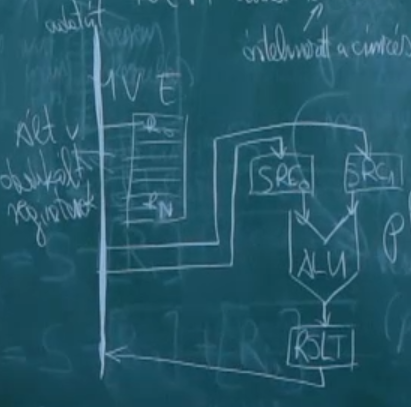
\includegraphics[width=0.8\textwidth]{adatut}
    \centering
    \caption{Egyutas adatút}
    \label{fig:adatut}
\end{figure}
Példa egyutas adatút működésére ADD r0,r1 művelet esetén:
\begin{enumerate}
    \item Az R0 tartalmát be kell tölteni az egyik forrásregiszterbe, ezért a vezérlő megnyitja R0 és SRC0 kapcsolóit, hogy az adatúton keresztül a jel eljuthasson.
    \item Ezután jön R1, itt R1 és SRC1 kapcsolóit nyitja a vezérlő.
    \item Szinkronizáltan, órajelre megnyílnak SRC0 és SRC1 kimenő kapcsolói, a forrás operandusok eljutnak az ALU-ba, ahol megtörténik az összeadás.
    \item Az ALU-ból bekerül az adat az eredményregiszterbe.
    \item Végül az eredmény visszajut R0-ba.
\end{enumerate}

\subsubsection{Kétutas csatolás}
A kétutas csatolás használatával egyszerre tölthető be a két operandus, így a betöltési idő a felére csökken.
\begin{figure}[H]
    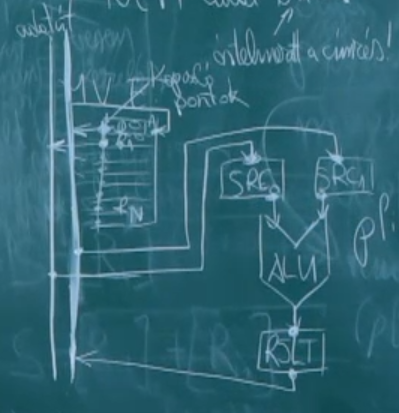
\includegraphics[width=0.8\textwidth]{ketut}
    \centering
    \caption{Kétutas adatút}
    \label{fig:ketut}
\end{figure}

\subsubsection{Háromutas csatolás}
Itt a harmadik adatút a kimenetre van rákötve.
Ezzel párhuzamos működés érhető el: a visszaírással együtt megtörténhet a következő utasítás forrás operandusainak betöltése.
\begin{figure}[H]
    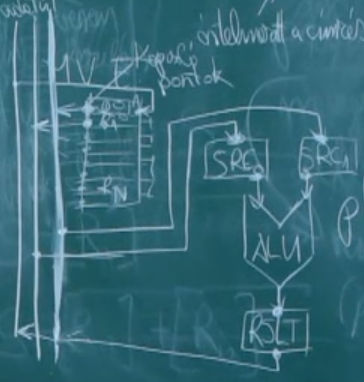
\includegraphics[width=0.8\textwidth]{haromut}
    \centering
    \caption{Háromutas adatút}
    \label{fig:haromut}
\end{figure}

\subsection{Műveletvégző (ALU)}
Az ALU (Aritmetikai Logikai Egység) végzi el a műveleteket.
A leggyakoribb, legelemibb művelet az összeadás.

\subsubsection{Az ALU által végzett műveletek}
\begin{itemize}
    \item FX: + - * /
    \item FP: + - * /
    \item BCD: + - * /
    \item Egyéb: eltolás, negálás, léptetés, logikai műveletek
\end{itemize}

\subsubsection{Összeadó}
Egy félösszeadónak két bemenete és két kimenete van, a második kimenet az átvitelre van (carry).
\begin{figure}[H]
    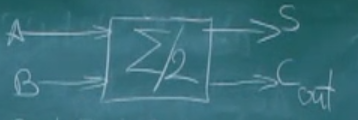
\includegraphics[width=0.8\textwidth]{felossze}
    \centering
    \caption{Félösszeadó}
    \label{fig:felossze}
\end{figure}
A carry bit meghatározásához egy AND kaput használ a félösszeadó (akkor van átvitel, ha mindkét bement 1), az ereményhez pedig egy XOR kaput.
\begin{figure}[H]
    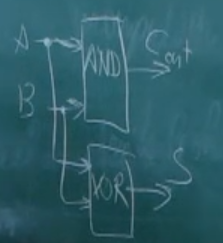
\includegraphics[width=0.8\textwidth]{felosszek}
    \centering
    \caption{Félösszeadó kapujainak felépítése}
    \label{fig:felosszek}
\end{figure}

Teljes összeadónál három bemenet van, hogy az előző összeadás carry kimenetét is figyelembe tudja venni.
\begin{figure}[H]
    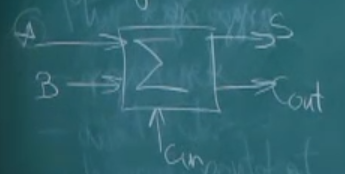
\includegraphics[width=0.8\textwidth]{teljesossze}
    \centering
    \caption{Teljes összeadó}
    \label{fig:teljesossze}
\end{figure}
A teljes összeadó felépíthető félösszeadókból:
\begin{figure}[H]
    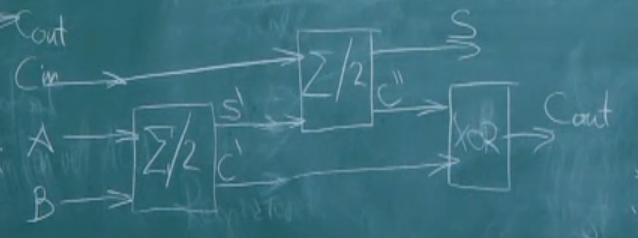
\includegraphics[width=0.8\textwidth]{teljesosszefel}
    \centering
    \caption{Teljes összeadó félösszeadókból}
    \label{fig:teljesosszefel}
\end{figure}
Ez 3 ciklusba kerül, a cél a folyamat gyorsítása.
Az igazságtáblát felírva és a logikai függvényeket egyszerűsítve a következő kapukból építhető fel a teljes összeadó:
\begin{figure}[H]
    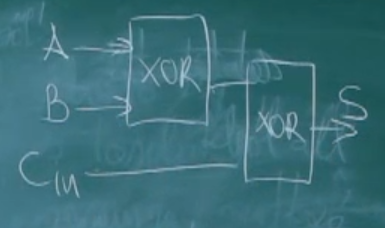
\includegraphics[width=0.8\textwidth]{teljesosszeegyszeru}
    \centering
    \caption{Teljes összeadó egyszerűsítése (eredmény kiszámítása)}
    \label{fig:teljesosszeegyszeru}
\end{figure}
\begin{figure}[H]
    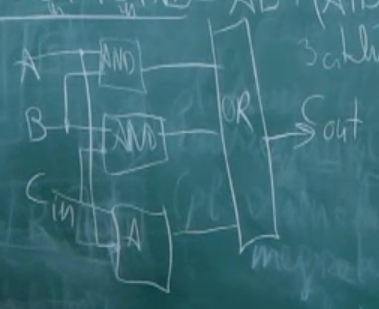
\includegraphics[width=0.8\textwidth]{teljesosszeegyszeruc}
    \centering
    \caption{Teljes összeadó egyszerűsítése (carry kiszámítása)}
    \label{fig:teljesosszeegyszeruc}
\end{figure}
Ezzel a művelet már két óraciklus alatt is elvégezhető, azaz a teljesítmény 33\%-kal növekszik.

\subsubsection{n-bites összeadó}
A gyakorlatban viszont általában nem biteket, hanem bitsorozatokat kell összeadni.
Ezeknek a bitsorozatoknak a tárolása regiszterekben történik (byte, szó, duplaszó).
A feladat tehát 2 db n-bites regiszter összeadása.

Az első ilyen megoldás az n-bites soros összeadó volt.
Ez a különböző helyiértékeken lévő biteket egymás után, külön-külön adja össze.
A carry-t is figyelembe veszi, ezt a flip-flopok tárolják.
Képes két különböző hosszú szám összeadására, ilyenkor a rövidebb számot automatikusan kiegészíti 0 helyiértékekkel.
A megvalósításhoz egy darab teljes összeadót használ, valamint bevezették a léptető regisztert.

A B léptető regiszter kimenete rá van vezetve a bemenetére.
A teljes összeadó bemenete a két léptető regiszter kimenetére csatlakozik.
Így a léptető regiszter kimenete minden alkalommal bekerül a teljes összeadóba és a B léptető regiszter bemenetére is.
Ekkor minden helyiérték egyel jobbra lép, a B regiszter tartalma változatlan marad, az A regiszterbe pedig bekerül az összeadás ereménye az összeadó kimenetéről.
\begin{figure}[H]
    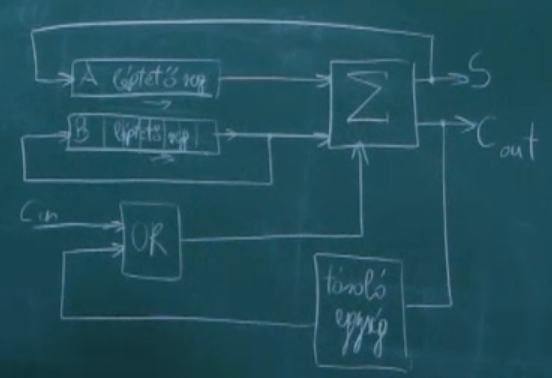
\includegraphics[width=0.8\textwidth]{lepteto}
    \centering
    \caption{n-bites soros összeadó és a léptető regiszterek}
    \label{fig:lepteto}
\end{figure}
A carry kezeléséhez a carry bementet először egy OR kapun kell átvezetni, így az előző összeadás carry-je és a bitenkénti összeadás carry-je is figyelembe van véve.
A tároló egység, a flip-flop feladata, hogy a carry bemenetet csak az első összeadásnál vegye figyelembe.

Ezzel a módszerrel az összeadás megtörtént, de a soros végrehajtás miatt viszonylag lassú.
Gyorsítási lehetőség az összeadás párhuzamosítása.
Ehhez n darab 1 bites összeadóra van szükség, amik bemeneteire a két bemeneti regiszter megfelelő bitjei vannak rákötve.
A teljes párhuzamos végrehajtást a carry bitek akadályozzák, mivel az n-edik bit előállításához szükség van az n-1-edik carry bit előállítására.
A végrehajtási idő tehát nem sokat javult, viszont amennyiben nincs carry, úgy nagyon gyorsan előáll az eredmény.
Tehát a végrehajtási idő hullámzó, a carry-től függ (ripple carry adder).

A további gyorsítás szimultán átvitelképzéssel lehetséges (carry lookahead - carry előrejelzés, más néven rekurzív módszer).
A carry kimenetet adó logikai függvény vizsgálatával kiderül, hogy a végeredmény nem függ a bitenkénti carrytől.
Az AB-t nevezzük generate-nek (G), az A+B-t propagate-nek (P).
Ezt felhasználva 3 kapu segítségével előállítható az összes carry.
Az ezt kiszámoló áramkör neve a CLA, azaz carry lookahead.
A CLA bemenete az A és B és a bemeneti carry.
Az összeadót úgy módosítjuk, hogy előállítsa P-t és G-t.
A teljes összeadó carry kimenetét nem használjuk, hanem azt a CLA állítja elő.
\begin{figure}[H]
    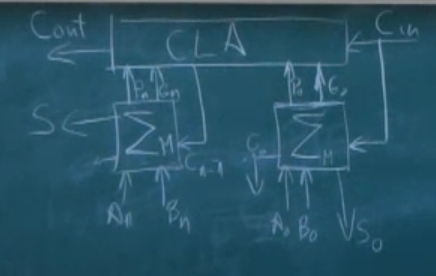
\includegraphics[width=0.8\textwidth]{cla}
    \centering
    \caption{A CLA-t használó összeadó felépítése}
    \label{fig:cla}
\end{figure}
Ezzel az összeadás 3 ciklus segítségével megvalósítható.
Korlátja, hogy egy OR kapu általában max 8 bemenetet kezel, tehát egy 32 bites összeadóhoz 4 db CLA-ra van szükség.
Ezt segíthetjük egy plusz CLA-val, ami a CLA-k bemenő carry-jeit állítja elő.

Az összes mai összeadó ilyen rekurzív módszerek szerint működik.

\subsubsection{Szorzás megvalósítása}
A szorzás is összeadások sorozatára vezethető vissza, így az előző módszerekkel megvalósítható.
Sok szorzásnál ez lassú, így itt is gyorsításra, egyszerűsítésre van szükség.

Az egyszerűsítéshez felhasználható az összeadás, invertálás és léptetés.
Régen ez gépi kódból történt, de manapság szakosodott műveletvégző egységek segítik ezeket a műveleteket.

Egyik egyszerűsítési lehetőség a gyűjtő regiszter és a léptetés használata.
A gyűjtőt a művelet előtt nullázzuk.

A szorzás eredménye általában több bit helyet foglal, tehát nem valószínű, hogy belefér a forrásregiszterbe.
Kettes számrendszerben ha A szám n bit hosszú, B pedig m bit hosszú, akkor elmondható, hogy $A*B <= m+n$.
Két 8 bites szám esetén pl. az eredmény 16 bit hosszú lehet.

Gyorsítási lehetőségek:
\begin{itemize}
    \item bitcsoporttal történő szorzás: pl. $7*9=63$, azaz $0111*1001$ szorzásánál először 10-al, majd 01-el szorzunk. Ha a bitcsoport 00, a szorzandót nem kell a gyűjtőhöz adni, csak 2-t léptetünk balra. Ha 01, a gyűjtőhöz a szorzandó egyszeresét adjuk hozzá és kettőt léptetünk balra. 10-nál a kétszeresét adjuk hozzá, azaz balra léptetünk egyet, hozzáadjuk, majd balra léptetünk kettőt (ha folytatódik a szorzás). 11-nél a 3-szorosát kell hozzáadni, majd kettőt léptetni balra (ehhez általában a 4-szeresét adjuk hozzá és kivonjuk az egyszeresét).
    \item Booth-féle algoritmus: probléma, hogy ha a szorzóban sok 1-es van, akkor lassú a szorzás. Ennek a gyorsításához a szorzóhoz közeli számmal szorzunk, majd a különbséget kivonjuk. Pl. 62-vel szorzásnál 64-el szorzunk (6 léptetés balra), majd kivonjuk a szorzandó kétszeresét.
\end{itemize}

\subsubsection{Osztás}
Az osztás igényli a legtöbb időt, mivel bonyolult művelet.
Különbség, hogy itt két kimenet van, az eredmény és a maradék, valamint kivételek is felléphetnek.



